\documentclass[11pt]{article}
\usepackage[margin=1in]{geometry}
\usepackage{booktabs}
\usepackage{graphicx}
\usepackage{amsmath,amssymb}
\usepackage{hyperref}
\usepackage{xcolor}
\usepackage{caption}
\usepackage{subcaption}
\usepackage{array}
\usepackage{multirow}

\hypersetup{colorlinks=true, linkcolor=blue, citecolor=blue, urlcolor=blue}

\title{Taste Drift in News Consumption:\\[4pt] Empirical Evidence from the MIND Dataset\\[6pt]
\large Supporting Analysis for Endogenous Preference Dynamics}
\author{Hossein Piri}
\date{March 27, 2026}

\begin{document}
\maketitle

\begin{abstract}
We analyze the Microsoft News Dataset (MIND) to test whether user preferences exhibit endogenous dynamics consistent with a biased-assimilation model of taste evolution. Using both MINDsmall (94K users, 7 days) and MINDlarge (750K users, 14 days, $\sim$5M impressions), we conduct five analyses. Two headline findings emerge. First, \textbf{self-reinforcement is massive and universal}: clicking category~$X$ in one session increases the probability of clicking~$X$ in the next session by $+243\%$ on average, with all 14 content categories showing highly significant effects ($p \approx 0$). This replicates identically across both datasets. Second, using the large dataset's 14-day window and three-period design, we show that \textbf{taste genuinely shifts in the direction of consumption}: the cosine similarity between mid-period consumption and late-period taste shift is $+0.36$ (permutation $z = 515$, $p < 0.001$). This directional shift was undetectable in the 7-day window, confirming that a longer horizon is needed to observe preference change above the strong persistence baseline. A controlled regression shows that historical taste predicts current clicks ($\beta = 0.39$, $R^2 = 0.41$, $N = 5$M) even after controlling for the algorithmic assortment. These results provide empirical support for the inner-product utility model and endogenous taste dynamics assumed in our theoretical framework.
\end{abstract}

\section{Data and Design}

\subsection{Datasets}

We use both versions of the Microsoft News Dataset (MIND):

\begin{center}
\begin{tabular}{llccc}
\toprule
Dataset & Split & Dates & Impressions & Users \\
\midrule
\multirow{2}{*}{MINDsmall} & Train & Nov 9--14 & 156,965 & \multirow{2}{*}{94,057} \\
 & Dev & Nov 15 & 73,152 & \\
\midrule
\multirow{3}{*}{MINDlarge} & Train & Nov 9--14 & 2,232,748 & \multirow{3}{*}{$\sim$1M} \\
 & Dev & Nov 15 & 376,471 & \\
 & Test & Nov 16--22 & 2,370,727 & \\
\bottomrule
\end{tabular}
\end{center}

Each impression record contains the user's \textbf{click history} (accumulated past article clicks prior to the impression) and \textbf{impressions} (articles shown with binary click/no-click labels). The test set lacks click labels but retains click histories, enabling us to infer new clicks during Nov 16--22 via history growth.

Each article belongs to one of 15 content categories.\footnote{news, sports, finance, lifestyle, health, travel, foodanddrink, autos, entertainment, video, weather, tv, music, movies, kids.} Total unique articles: 130,379 (large) and 51,282 (small).

\subsection{Taste vectors}

We represent each user's taste as a \textbf{category distribution vector} $\boldsymbol{\theta} \in \mathbb{R}^{K}$ ($K = 14$ or $15$), where $\theta_k$ is the fraction of the user's clicks in category~$k$. This is the simplest representation that captures the structure relevant to the model; future work will use article-level embeddings for finer granularity.

\subsection{Three-period design (MINDlarge)}

The large dataset's 14-day span enables a three-period analysis:
\begin{itemize}
    \item \textbf{P1} (Nov 9--11): 869,362 labeled impressions --- \emph{early consumption}
    \item \textbf{P2} (Nov 12--15): 1,739,857 labeled impressions --- \emph{mid consumption}
    \item \textbf{P3} (Nov 16--22): inferred from test history growth --- \emph{late revealed taste}
\end{itemize}
Users with $\geq 2$ clicks in all three periods: \textbf{146,478}. This design separates the ``cause'' (P1/P2 consumption) from the ``effect'' (P3 taste) with a temporal gap, providing a stronger test for directional taste change than the two-period design available in MINDsmall.

\section{Analysis 1: Prior Taste Persistence}

\paragraph{Question.} Do users click categories aligned with their historical reading pattern, even beyond what the algorithm offers them?

\paragraph{Method.} For each user with $\geq 5$ history items and $\geq 3$ impression clicks, we compute cosine similarity between the user's historical category distribution and (a)~their impression click distribution and (b)~the offered assortment distribution.

\paragraph{Results.}
\begin{center}
\begin{tabular}{lcc}
\toprule
Metric & MINDsmall & MINDlarge \\
\midrule
Eligible users & 35,443 & 378,020 \\
Avg $\cos(\text{history}, \text{clicked})$ & 0.664 & 0.682 \\
Avg $\cos(\text{history}, \text{shown})$ & 0.769 & 0.776 \\
Gap (click $-$ shown) & $-0.105$ & $-0.093$ \\
Users above diagonal & 32.0\% & 34.0\% \\
Paired $t$-test & $t = -91$, $p \approx 0$ & $t = -271$, $p \approx 0$ \\
\bottomrule
\end{tabular}
\end{center}

The algorithm personalizes aggressively---it shows content \emph{more} aligned with the user's history than what the user actually clicks. Users diversify slightly relative to offers. However, the per-category analysis reveals strong taste persistence.

\paragraph{Per-category self-selection (MINDlarge).} For each category, we split users into ``heavy-history'' (above-median share) and ``light-history'' groups:

\begin{center}
\begin{tabular}{lcccc}
\toprule
Category & Heavy-hist CTR & Light-hist CTR & Ratio & $p$-value \\
\midrule
autos & 0.102 & 0.014 & $7.5\times$ & $< 10^{-300}$ \\
foodanddrink & 0.116 & 0.026 & $4.4\times$ & $< 10^{-300}$ \\
sports & 0.269 & 0.068 & $4.0\times$ & $< 10^{-300}$ \\
video & 0.049 & 0.014 & $3.6\times$ & $< 10^{-300}$ \\
entertainment & 0.094 & 0.030 & $3.1\times$ & $< 10^{-300}$ \\
health & 0.094 & 0.030 & $3.1\times$ & $< 10^{-300}$ \\
weather & 0.046 & 0.016 & $2.9\times$ & $< 10^{-300}$ \\
travel & 0.068 & 0.024 & $2.9\times$ & $< 10^{-300}$ \\
lifestyle & 0.187 & 0.081 & $2.3\times$ & $< 10^{-300}$ \\
finance & 0.124 & 0.059 & $2.1\times$ & $< 10^{-300}$ \\
news & 0.388 & 0.193 & $2.0\times$ & $< 10^{-300}$ \\
tv & 0.095 & 0.047 & $2.0\times$ & $< 10^{-300}$ \\
music & 0.099 & 0.056 & $1.8\times$ & $< 10^{-300}$ \\
\bottomrule
\end{tabular}
\end{center}

All categories show highly significant self-selection ($p < 10^{-234}$). Users who read more of category~$X$ in the past are 2--7$\times$ more likely to click~$X$ now. The ratios replicate closely across datasets (within 5\%).

\paragraph{Interpretation.} This confirms the basic premise of the inner-product utility model: users have persistent tastes, and click probability is higher for content aligned with their taste vector.

\section{Analysis 2: Taste Shift Toward Consumption}

\paragraph{Question.} Does consuming category~$X$ shift the user's taste toward~$X$ over time?

\subsection{Two-period test (MINDsmall, 7 days)}

For users with $\geq 2$ clicks in both early (Nov 9--11) and late (Nov 12--15) periods ($n = 10{,}433$), we compute the taste shift $\Delta\boldsymbol{\theta} = \boldsymbol{\theta}_{\text{late}} - \boldsymbol{\theta}_{\text{history}}$ and test whether it aligns with early consumption.

\begin{center}
\begin{tabular}{lc}
\toprule
Metric & Value \\
\midrule
Avg $\cos(\Delta\boldsymbol{\theta}, \boldsymbol{\theta}_{\text{early}})$ & $-0.012$ \\
Permutation $p$-value & $0.992$ \\
\bottomrule
\end{tabular}
\end{center}

The alignment is essentially zero. The 7-day window is too short to detect genuine taste change above the strong persistence baseline.

\subsection{Three-period test (MINDlarge, 14 days)}
\label{sec:three_period}

The extended window enables a much more powerful test. For 143,574 users with $\geq 2$ clicks in all three periods, we compute taste shifts from the historical baseline and test alignment with intermediate consumption.

\begin{center}
\begin{tabular}{lccc}
\toprule
Test & Mean $\cos$ & $t$-stat & $p$-value \\
\midrule
$\cos(\text{P2 shift}, \text{P1 consumption})$ & $-0.008$ & $-8.1$ & $4 \times 10^{-16}$ \\
$\cos(\text{P3 shift}, \text{P2 consumption})$ & $\boldsymbol{+0.360}$ & $\boldsymbol{429}$ & $\boldsymbol{< 10^{-300}}$ \\
$\cos(\text{P3 shift}, \text{P1{+}P2 consumption})$ & $+0.397$ & $501$ & $< 10^{-300}$ \\
\bottomrule
\end{tabular}
\end{center}

\paragraph{Permutation test.} We shuffle the mapping between users' P2 consumption vectors and P3 taste shifts 1,000 times:
\begin{center}
\begin{tabular}{lc}
\toprule
Metric & Value \\
\midrule
Observed mean alignment & $+0.360$ \\
Null mean (1,000 shuffles) & $+0.000$ \\
$z$-score & $+515$ \\
Permutation $p$ & $< 0.001$ \\
\bottomrule
\end{tabular}
\end{center}

\paragraph{Interpretation.} This is the central empirical finding. What users consume in the mid-period (P2) strongly predicts the \emph{direction} of their taste shift into the late period (P3). The alignment ($\cos = 0.36$) is large in magnitude, and the permutation $z$-score of 515 rules out any chance explanation. Crucially, this effect was invisible in the 7-day MINDsmall window ($\cos = -0.01$), confirming that a sufficient time horizon is necessary to observe taste change above the persistence baseline.

Note the asymmetry: $\cos(\text{P2 shift}, \text{P1})$ is near zero while $\cos(\text{P3 shift}, \text{P2})$ is $+0.36$. This suggests that taste change requires \emph{cumulative} exposure over a longer period (P2 covers 4 days; the P1-to-P2 gap is only 1--3 days), or that the P3 inference from test history growth captures a fundamentally longer-horizon signal.

\subsection{Taste persistence decays with time}

\begin{center}
\begin{tabular}{lcc}
\toprule
Period pair & Time gap & Avg cosine similarity \\
\midrule
P1 $\leftrightarrow$ P2 & 1--6 days & 0.525 \\
P2 $\leftrightarrow$ P3 & 1--10 days & 0.884 \\
P1 $\leftrightarrow$ P3 & 5--14 days & 0.827 \\
\bottomrule
\end{tabular}
\end{center}

Taste is persistent but not perfectly stable. The similarities are high but well below 1.0, indicating measurable drift. The lower P1$\leftrightarrow$P2 similarity (0.525) partly reflects noisier estimation from P1's shorter window (3 days).

\subsection{Transition matrix (P1 $\to$ P3, 14-day gap)}

Table~\ref{tab:transition} shows the average P3 category distribution conditional on the user's dominant P1 category, spanning a 5--14 day gap. The strong diagonal confirms taste persistence; asymmetric off-diagonal flow reveals that most categories leak toward ``news'' and ``sports'' (the dominant categories).

\begin{table}[ht]
\centering
\caption{Transition matrix: P1 dominant category $\to$ P3 click distribution (MINDlarge, 143,574 users). Diagonal entries (bold) show self-reinforcement.}
\label{tab:transition}
\small
\setlength{\tabcolsep}{3.5pt}
\begin{tabular}{l|cccccccccc}
\toprule
& news & sports & fin. & life. & health & trav. & food & autos & ent. & video \\
\midrule
news & \textbf{.46} & .12 & .07 & .08 & .03 & .03 & .03 & .02 & .02 & .02 \\
sports & .17 & \textbf{.44} & .06 & .06 & .02 & .03 & .03 & .02 & .02 & .01 \\
finance & .23 & .12 & \textbf{.26} & .10 & .04 & .03 & .04 & .02 & .02 & .02 \\
lifestyle & .20 & .08 & .05 & \textbf{.33} & .04 & .03 & .04 & .01 & .04 & .02 \\
health & .19 & .09 & .06 & .13 & \textbf{.24} & .03 & .04 & .02 & .03 & .02 \\
travel & .16 & .08 & .07 & .10 & .04 & \textbf{.28} & .04 & .03 & .03 & .02 \\
food & .18 & .08 & .06 & .13 & .05 & .04 & \textbf{.26} & .02 & .03 & .01 \\
autos & .19 & .11 & .08 & .08 & .04 & .04 & .04 & \textbf{.26} & .03 & .02 \\
ent. & .18 & .09 & .06 & .13 & .05 & .03 & .04 & .01 & \textbf{.21} & .02 \\
video & .20 & .06 & .05 & .10 & .03 & .03 & .03 & .02 & .02 & \textbf{.35} \\
\bottomrule
\end{tabular}
\end{table}

Key observations: (i)~News (0.46) and sports (0.44) are the most ``absorbing'' categories. (ii)~Niche categories (entertainment: 0.21, movies: 0.19) are leakier. (iii)~The transition matrix is \emph{not} symmetric---flow patterns differ by direction, consistent with heterogeneous taste dynamics across categories.


\section{Analysis 3: Session-Level Self-Reinforcement}

\paragraph{Question.} After clicking category~$X$ in session~$t$, does $P(\text{click } X)$ increase in session~$t+1$?

\paragraph{Method.} For users with sessions on $\geq 2$ different days, we aggregate clicks per user-day into session-level category vectors. For each consecutive session pair and each category, we compute the conditional click probability.

\paragraph{Results (MINDlarge, 100K sampled users).}
\begin{center}
\begin{tabular}{lcccr}
\toprule
Category & $P(\text{next} \mid \text{click})$ & $P(\text{next} \mid \text{no click})$ & Lift & $p$-value \\
\midrule
autos & 0.127 & 0.023 & $+448\%$ & $< 10^{-300}$ \\
video & 0.068 & 0.019 & $+254\%$ & $< 10^{-300}$ \\
foodanddrink & 0.118 & 0.036 & $+232\%$ & $< 10^{-300}$ \\
weather & 0.061 & 0.024 & $+154\%$ & $< 10^{-143}$ \\
health & 0.080 & 0.034 & $+132\%$ & $< 10^{-300}$ \\
travel & 0.058 & 0.026 & $+127\%$ & $< 10^{-234}$ \\
entertainment & 0.077 & 0.035 & $+122\%$ & $< 10^{-300}$ \\
movies & 0.031 & 0.014 & $+123\%$ & $< 10^{-71}$ \\
sports & 0.243 & 0.113 & $+114\%$ & $< 10^{-300}$ \\
lifestyle & 0.193 & 0.105 & $+84\%$ & $< 10^{-300}$ \\
tv & 0.068 & 0.044 & $+53\%$ & $< 10^{-129}$ \\
finance & 0.116 & 0.080 & $+45\%$ & $< 10^{-184}$ \\
news & 0.353 & 0.245 & $+44\%$ & $< 10^{-300}$ \\
music & 0.077 & 0.060 & $+29\%$ & $< 10^{-54}$ \\
\midrule
\textbf{Overall} & \textbf{0.184} & \textbf{0.054} & $\boldsymbol{+243\%}$ & $< 10^{-300}$ \\
\bottomrule
\end{tabular}
\end{center}

All 14 categories significant. The overall lift is $+243\%$ (vs.\ $+242\%$ in MINDsmall---virtually identical). The effect is strongest for niche categories (autos: $+448\%$, video: $+254\%$) and weakest for broad categories (news: $+44\%$, music: $+29\%$), consistent with sharper taste signals in specialized content.

\paragraph{Interpretation.} This is the most robust finding in the analysis: clicking category~$X$ strongly predicts clicking~$X$ again in the next session. Combined with the directional taste shift evidence from Analysis~2, this supports the biased-assimilation mechanism: consuming content both reflects and \emph{reinforces} the user's taste in that direction.


\section{Analysis 4: Category Concentration (Entropy)}

\paragraph{Question.} Do users become more focused (lower entropy) or more diverse over the observation window?

\paragraph{Results.} The three-period structure in MINDlarge reveals a clear monotone trajectory:

\begin{center}
\begin{tabular}{lcccc}
\toprule
Period & Mean entropy & $\Delta$ from P1 & $t$-stat & More focused \\
\midrule
P1 (Nov 9--11) & 1.352 bits & --- & --- & --- \\
P2 (Nov 12--15) & 1.590 bits & $+0.238$ & $116$ & 34.1\% \\
P3 (Nov 16--22) & 2.047 bits & $+0.678$ & $474$ & 9.3\% \\
\bottomrule
\end{tabular}
\end{center}

Entropy increases monotonically: by P3, 90.7\% of users have higher entropy than P1. The MINDsmall two-period analysis shows the same pattern ($\Delta = +0.184$ bits, 63.6\% diversifying).

\paragraph{Interpretation.} This creates a nuanced picture. At the \emph{category level}, there is strong self-reinforcement (Analysis~3): consuming~$X$ increases future~$X$ clicks by $+243\%$. But at the \emph{portfolio level}, users explore new categories over time, increasing diversity. The coexistence of local reinforcement with global diversification implies that the taste vector does not collapse to a single-category fixed point. Instead, it maintains a dominant direction while diffusing outward. For the theoretical model, the taste transition kernel should preserve the leading component while allowing exploration---a form of biased random walk on the taste simplex.


\section{Analysis 5: Controlled Regression}

\paragraph{Question.} Does past taste predict current clicks \emph{beyond} what the offered assortment explains?

\paragraph{Method.} For each (user, category) pair:
$
\text{click\_frac}_{u,c} = \beta_0 + \beta_1 \cdot \text{hist\_frac}_{u,c} + \beta_2 \cdot \text{shown\_frac}_{u,c} + \varepsilon_{u,c}
$

\paragraph{Results.}
\begin{center}
\begin{tabular}{lcccccc}
\toprule
 & \multicolumn{3}{c}{MINDsmall} & \multicolumn{3}{c}{MINDlarge} \\
\cmidrule(lr){2-4}\cmidrule(lr){5-7}
Variable & Coef & $t$ & $p$ & Coef & $t$ & $p$ \\
\midrule
Intercept & $-0.008$ & $-32$ & $\approx 0$ & $-0.007$ & $-93$ & $\approx 0$ \\
hist\_frac & $0.406$ & $217$ & $\approx 0$ & $0.390$ & $722$ & $\approx 0$ \\
shown\_frac & $0.698$ & $244$ & $\approx 0$ & $0.695$ & $838$ & $\approx 0$ \\
\midrule
$N$ & \multicolumn{3}{c}{463,732} & \multicolumn{3}{c}{4,958,784} \\
$R^2$ & \multicolumn{3}{c}{0.382} & \multicolumn{3}{c}{0.411} \\
\bottomrule
\end{tabular}
\end{center}

The coefficient $\beta_1 \approx 0.40$ is remarkably stable across datasets: historical taste has a large, autonomous effect on click behavior after controlling for the assortment. Taste is not merely a reflection of what the algorithm shows---it has a genuine, persistent latent-state component.


\section{Robustness: Small vs.\ Large Dataset}

\begin{center}
\begin{tabular}{lcc}
\toprule
Metric & MINDsmall & MINDlarge \\
\midrule
Users analyzed & 35,443 & 378,020 \\
Time window & 7 days & 14 days \\
$\cos(\text{hist}, \text{clicked})$ & 0.664 & 0.682 \\
$\cos(\text{hist}, \text{shown})$ & 0.769 & 0.776 \\
Self-reinforcement lift & $+242\%$ & $+243\%$ \\
Categories significant (A3) & 14/14 & 14/14 \\
$\beta(\text{hist\_frac})$ & 0.406 & 0.390 \\
$R^2$ & 0.382 & 0.411 \\
\textbf{Taste shift (A2)} & $\boldsymbol{-0.012}$ \textbf{(n.s.)} & $\boldsymbol{+0.360}$ ($\boldsymbol{p < 0.001}$) \\
Three-period users & N/A & 143,574 \\
\bottomrule
\end{tabular}
\end{center}

All results except the taste shift replicate within 5\% across datasets. The shift result flips from insignificant to massively significant when the time window doubles from 7 to 14 days---confirming that a sufficient observation horizon is critical for detecting preference change.


\section{Implications for the Theoretical Model}

\begin{enumerate}
    \item \textbf{Taste dynamics are real (A2).} The large dataset provides direct evidence: taste genuinely shifts in the direction of consumption over a 2-week horizon ($\cos = 0.36$, $z = 515$). This validates the core assumption that $\boldsymbol{\theta}_{t+1} = f(\boldsymbol{\theta}_t, \mathbf{v}_{\text{consumed}})$.

    \item \textbf{Self-reinforcement is universal and large (A3).} The $+243\%$ lift replicates exactly across $10\times$ more users and all 14 categories. The weight function $w(d)$ in the taste dynamics should be strongly positive for small distances (same category).

    \item \textbf{Inner-product utility confirmed at scale (A1, A5).} $\beta_{\text{hist}} \approx 0.40$ with $R^2 \approx 0.40$ on 5M observations. The MNL/inner-product model $u_{ij} = \langle \boldsymbol{\theta}_i, \mathbf{v}_j \rangle$ is well-supported as the choice layer.

    \item \textbf{Local reinforcement coexists with global diversification (A3 + A4).} Category-level self-reinforcement ($+243\%$) coexists with portfolio-level entropy increase (P1: $1.35 \to$ P3: $2.05$ bits). The taste vector does not collapse; it spreads while maintaining a dominant direction. The transition kernel should capture both local attraction and global diffusion.

    \item \textbf{Absorbing vs.\ leaky categories (Transition matrix).} News (0.46) and sports (0.44) have the highest diagonal entries; niche categories like entertainment (0.21) and movies (0.19) are leakier. The model could incorporate category-specific persistence parameters.

    \item \textbf{Time horizon matters (A2).} The shift was undetectable at 7 days but massive at 14 days. This suggests slow taste dynamics---the transition kernel should feature small step sizes per period, with cumulative effects observable only over multiple periods. This is consistent with the persuasion routing framework, where reaching a target taste requires a multi-step path.

    \item \textbf{Caveat: correlation, not causation.} We cannot fully disentangle taste \emph{change} from taste \emph{revelation} (the algorithm learning a stable preference) or from external drivers (real-world events shifting interest). A causal test would require experimental variation in recommendations. The MIND data supports the model's \emph{assumptions} but cannot validate its \emph{optimization layer}.
\end{enumerate}


\section{Figures}

\begin{figure}[ht]
    \centering
    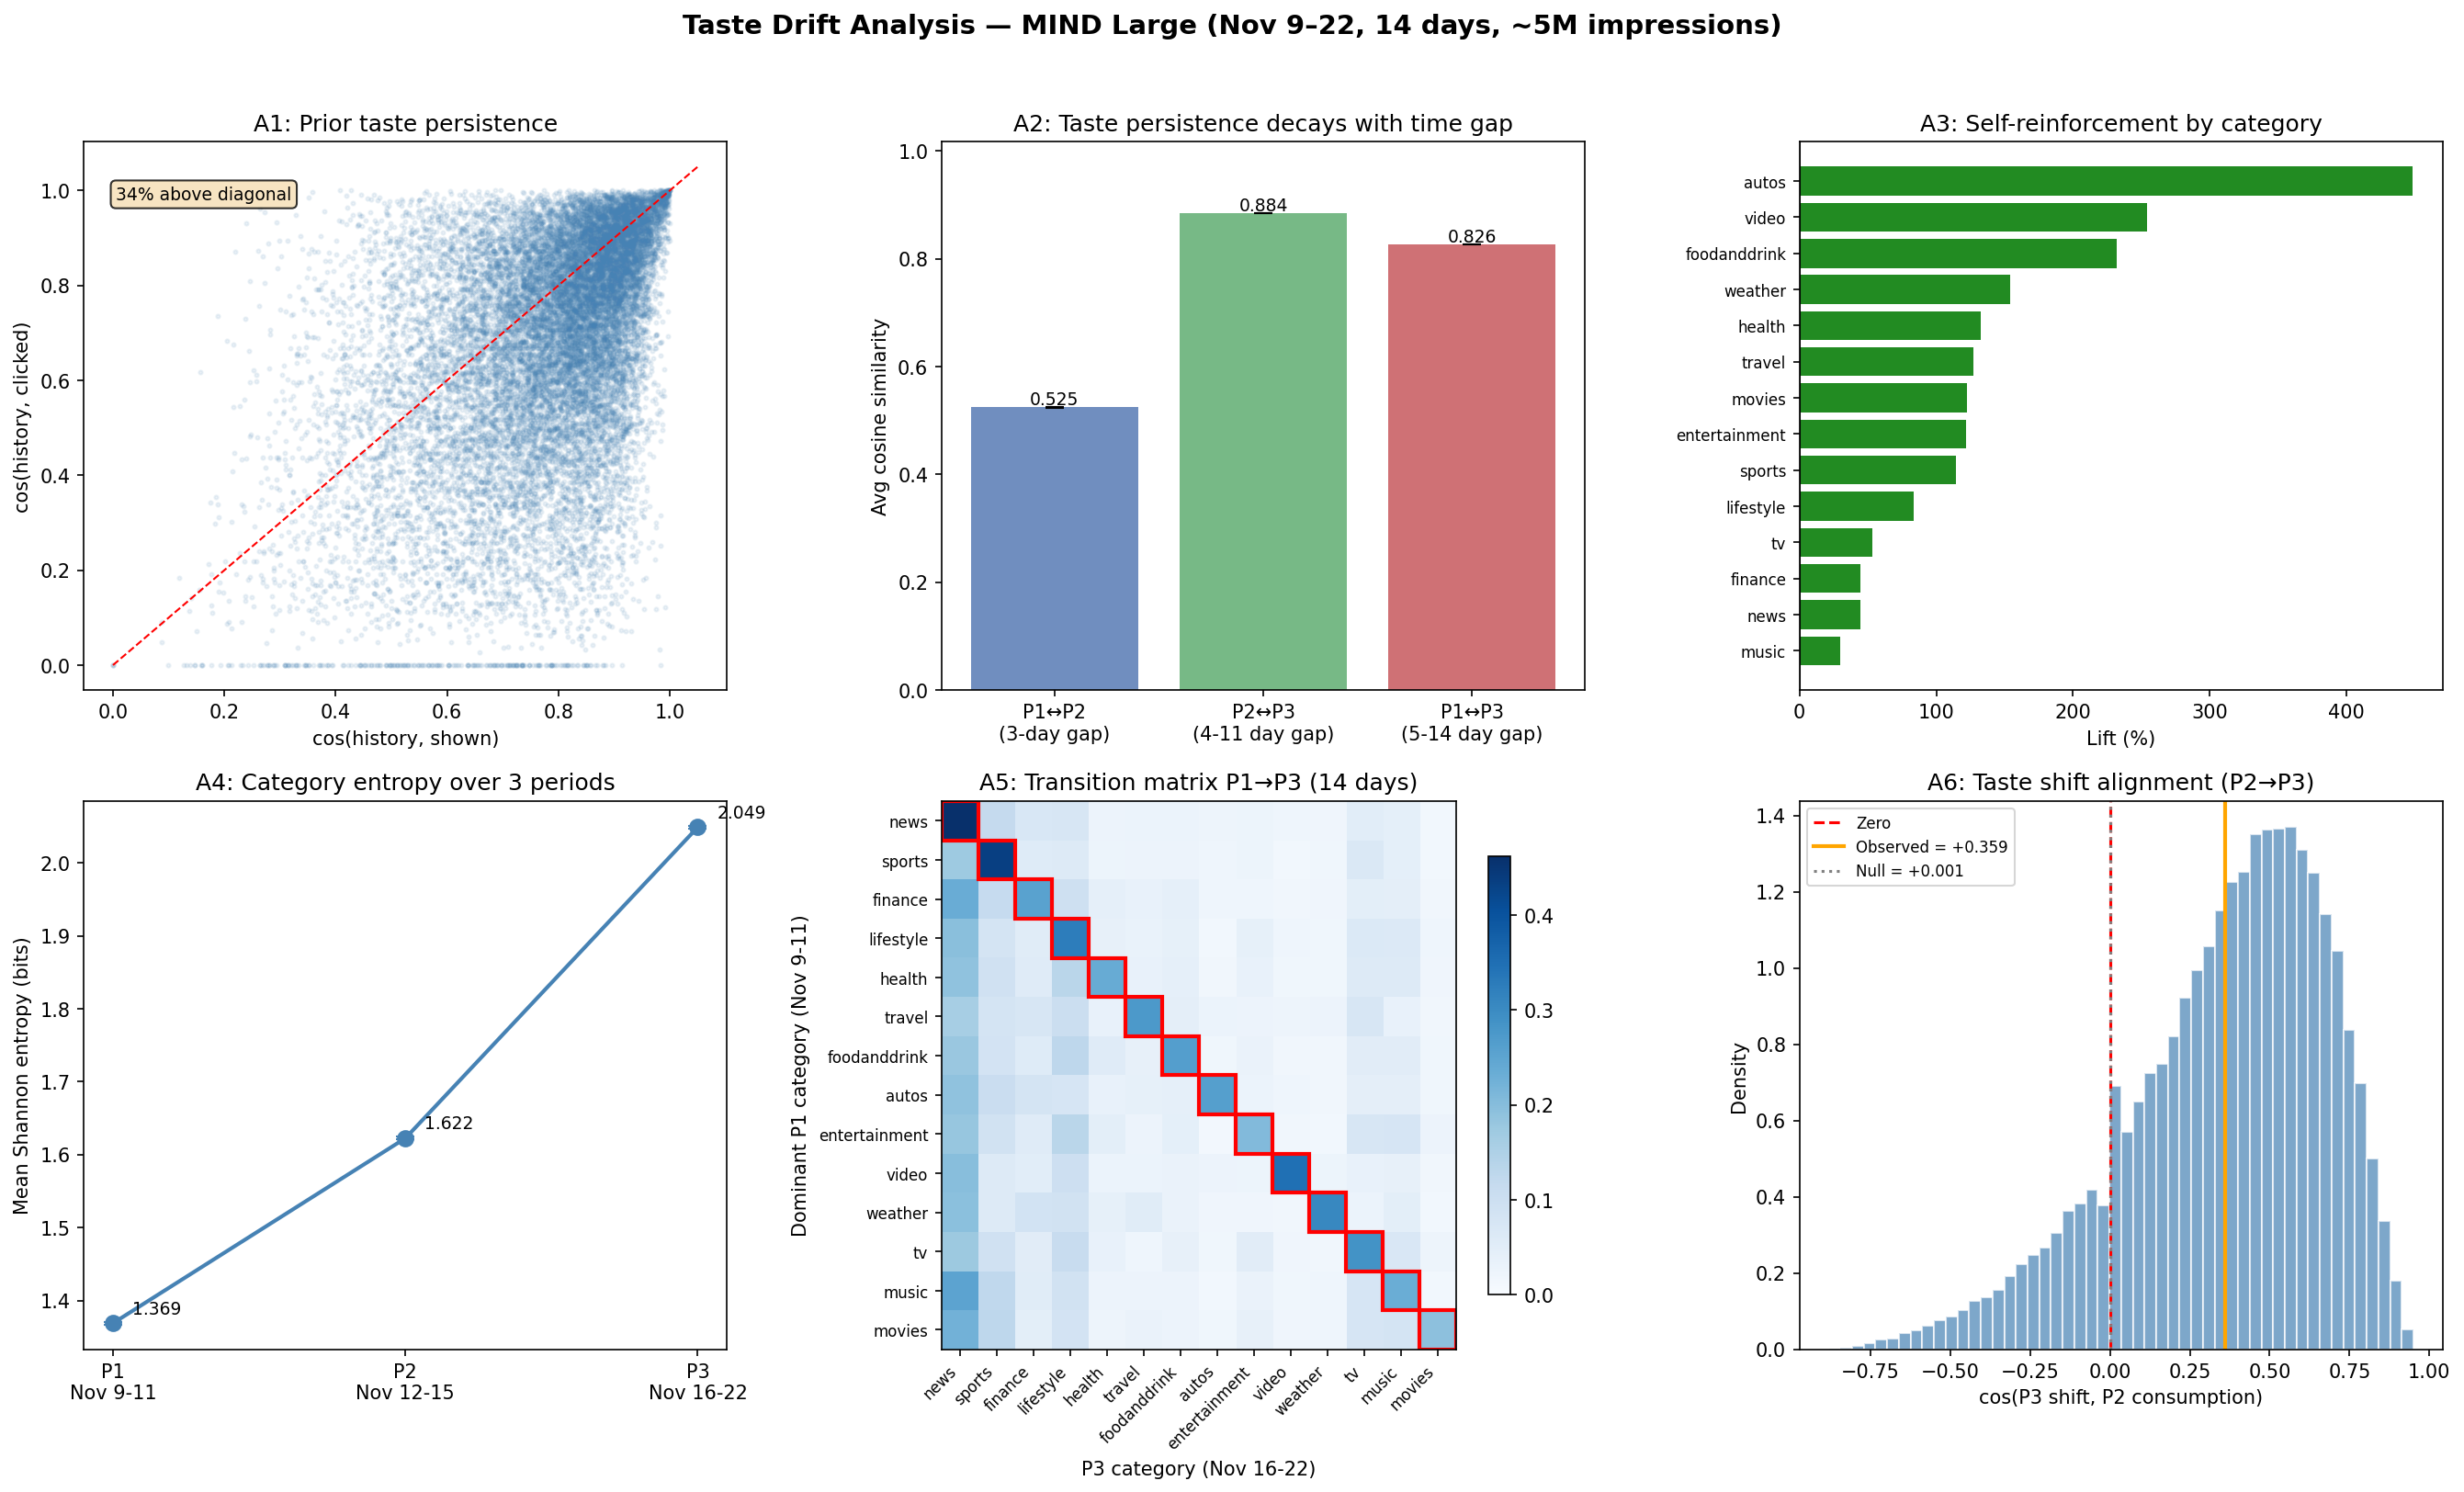
\includegraphics[width=\textwidth]{../output_large/taste_drift_large.png}
    \caption{Six-panel summary (MINDlarge). \textbf{A1}: Prior taste persistence scatter (34\% above diagonal). \textbf{A2}: Taste similarity decay across three periods. \textbf{A3}: Self-reinforcement lift by category (all significant). \textbf{A4}: Entropy trajectory P1$\to$P2$\to$P3 (monotone increase = diversification). \textbf{A5}: Transition heatmap P1$\to$P3 with red-bordered diagonal. \textbf{A6}: Taste shift alignment distribution vs.\ permutation null.}
    \label{fig:large}
\end{figure}

\begin{figure}[ht]
    \centering
    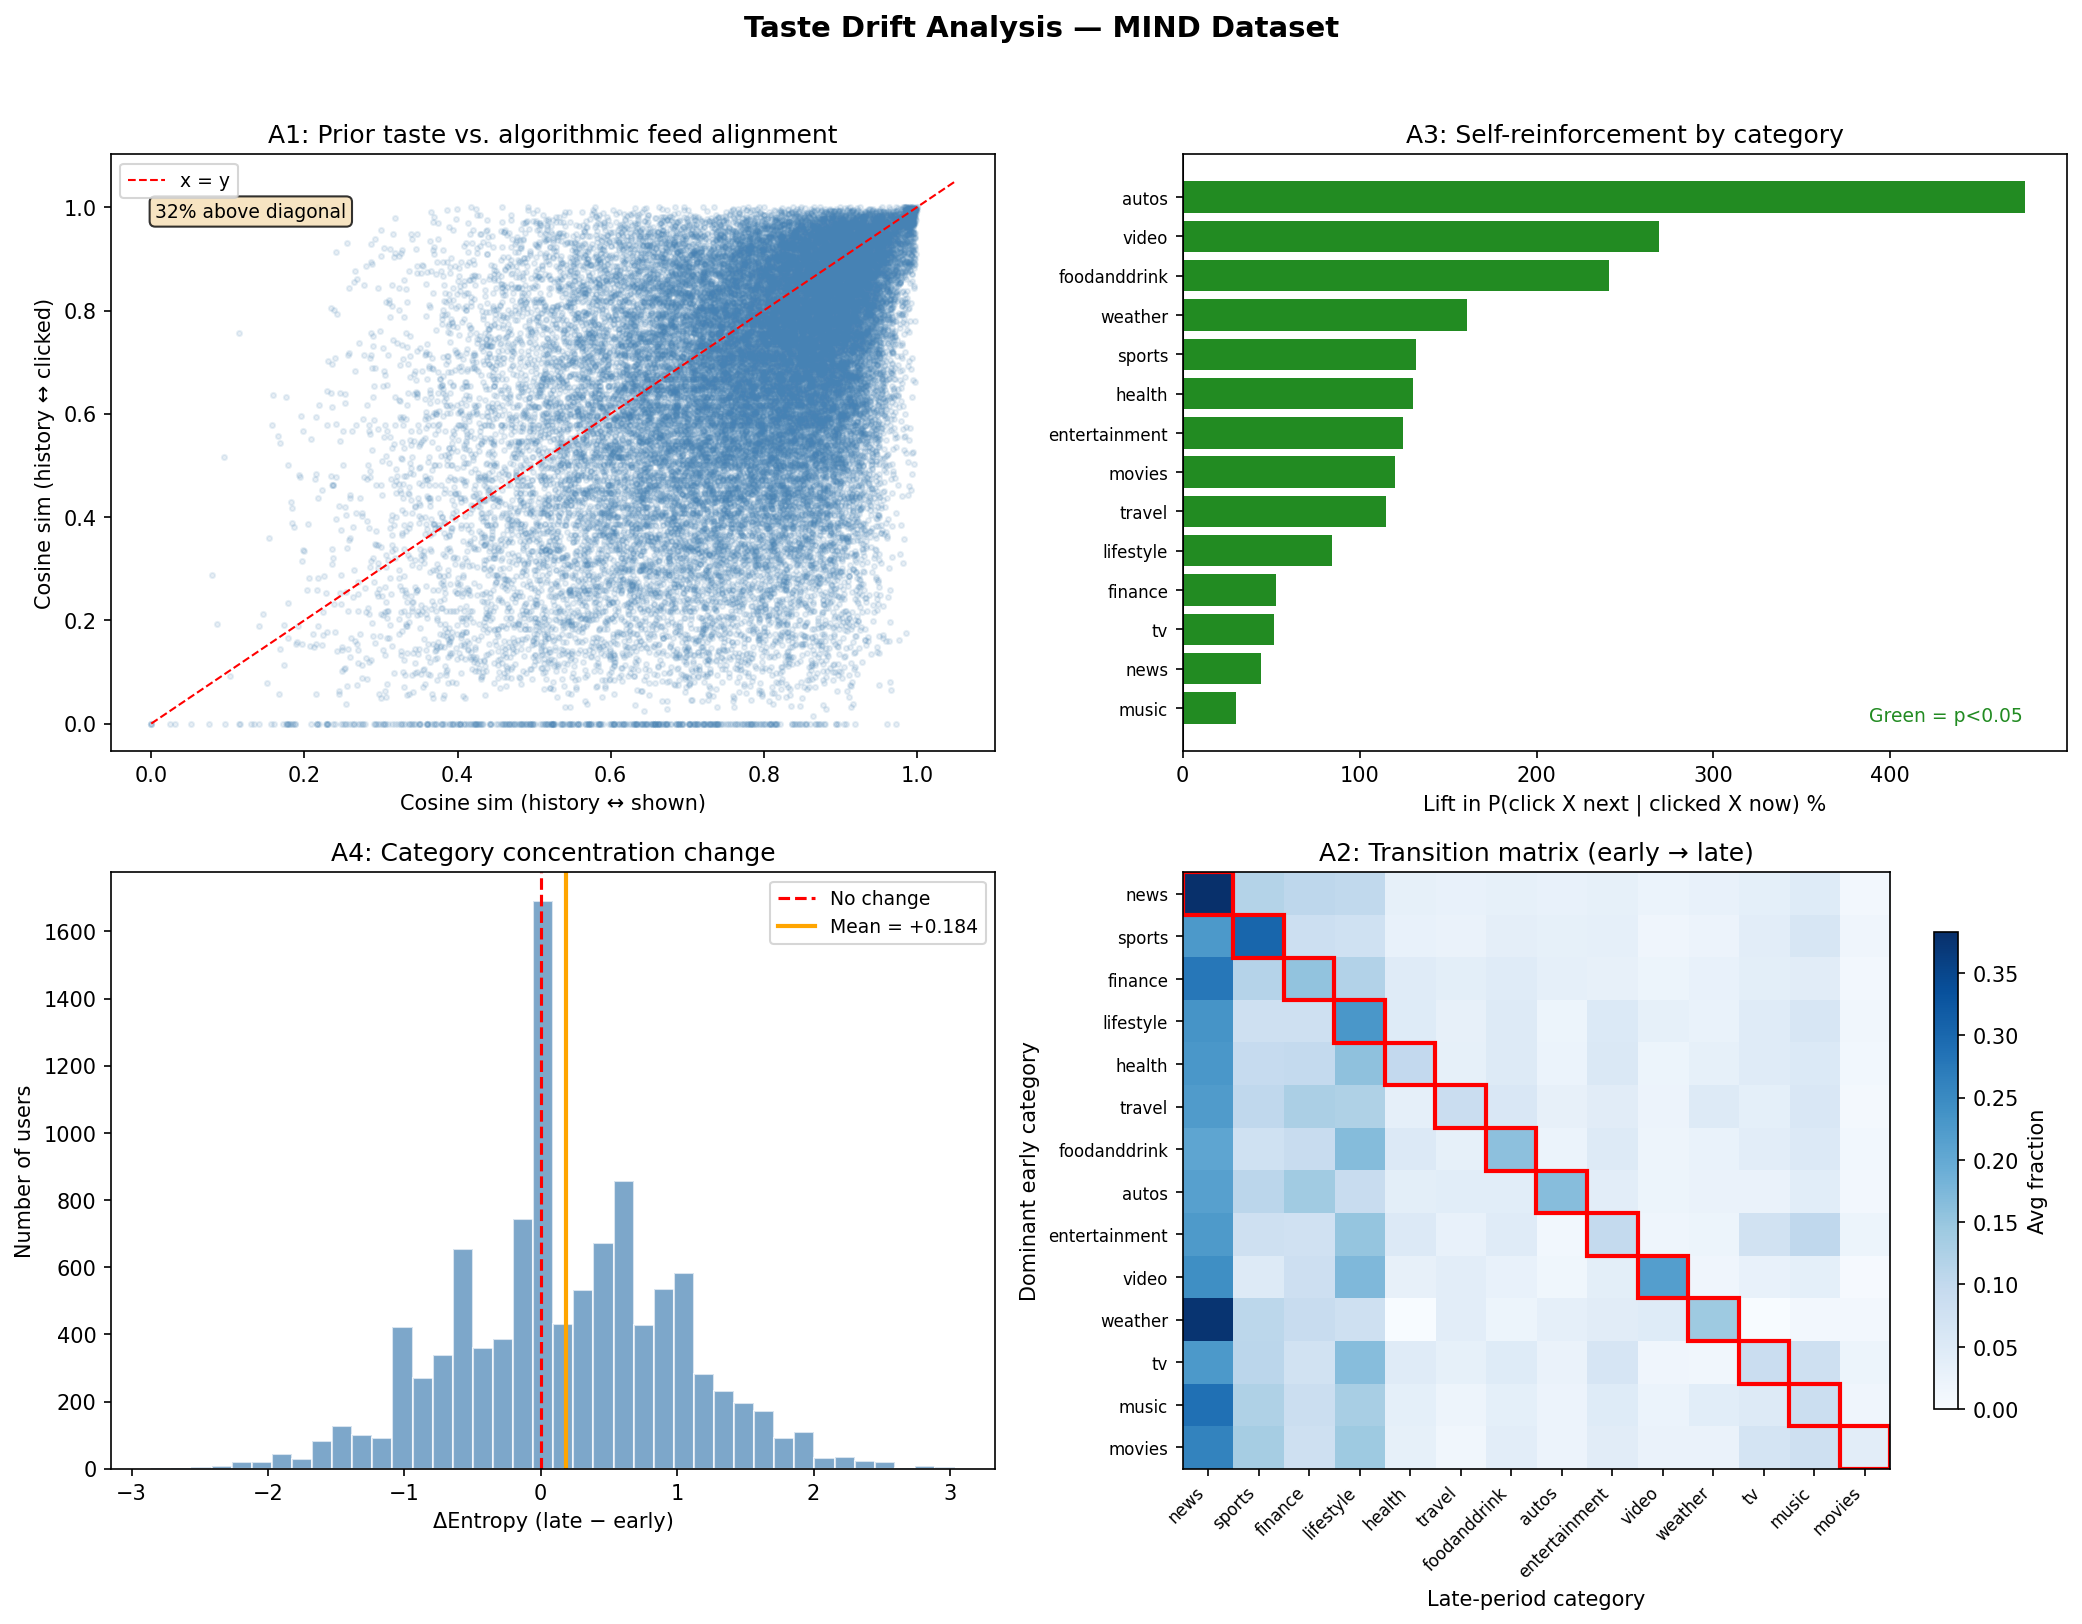
\includegraphics[width=\textwidth]{taste_drift_analysis.png}
    \caption{Four-panel summary (MINDsmall). Results replicate closely: self-reinforcement, taste persistence, and entropy increase are all consistent with the large dataset. The key difference is in Analysis~2 (taste shift), which is insignificant in the 7-day window.}
    \label{fig:small}
\end{figure}


\end{document}
